\chapter{Causal inference}\label{chap12}

\section*{Solutions of Exercises}\label{sec12_1}
\begin{enumerate}[leftmargin=*]
\item Show that the Average Treatment Effect (ATE) in the simple linear regression framework
\[
Y_i = \beta_0 + \tau D_i + \mu_i,
\]
assuming non-informative prior distributions, so that the posterior mean of the location parameter coincides with the maximum likelihood estimator, is equal to
\[
\bar{y}_1 - \bar{y}_0.
\]

\textbf{Answer}

Consider the simple linear regression model
\[
Y_i = \beta_0 + \tau D_i + \mu_i, \qquad i = 1,\dots,N,
\]
where $D_i \in \{0,1\}$ is a treatment indicator. In matrix notation:
\[
\mathbf{y} = X \boldsymbol{\beta} + \boldsymbol{\mu}, \qquad
X = \begin{pmatrix}
	1 & D_1 \\
	\vdots & \vdots \\
	1 & D_n
\end{pmatrix}, \quad
\boldsymbol{\beta} = \begin{pmatrix}\beta_0 \\ \tau \end{pmatrix}.
\]

Under the usual Gaussian likelihood and a non-informative prior $\pi(\boldsymbol{\beta},\sigma^2) \propto \sigma^{-2}$, the posterior mean of $\boldsymbol{\beta}$ coincides with the maximum likelihood estimator (MLE), which is the ordinary least squares (OLS) estimator:
\[
\widehat{\boldsymbol{\beta}} = (\mathbf{X}^\top \mathbf{X})^{-1} \mathbf{X}^\top \mathbf{y}.
\]

Compute $\mathbf{X}^\top \mathbf{X}$ and $\mathbf{X}^\top \mathbf{y}$:
\[
\mathbf{X}^\top \mathbf{X} =
\begin{pmatrix}
	N & N_1 \\
	N_1 & N_1
\end{pmatrix}, \qquad
\mathbf{X}^\top \mathbf{y} =
\begin{pmatrix}
	\sum_{i=1}^N y_i \\
	\sum_{i:D_i=1} y_i
\end{pmatrix},
\]
where $N_1 = \sum_i D_i$ and $N_0 = N - N_1$. Let $\bar{y}_1 = \frac{1}{N_1}\sum_{i:D_i=1} y_i$ and $\bar{y}_0 = \frac{1}{N_0}\sum_{i:D_i=0} y_i$.

Compute the inverse:
\[
(\mathbf{X}^\top \mathbf{X})^{-1} =
\frac{1}{N_0 N_1}
\begin{pmatrix}
	N_1 & -N_1 \\
	-N_1 & N
\end{pmatrix}.
\]

Thus:
\[
\widehat{\boldsymbol{\beta}} =
\frac{1}{N_0 N_1}
\begin{pmatrix}
	N_1 & -N_1 \\
	-N_1 & N
\end{pmatrix}
\begin{pmatrix}
	\sum_{i=1}^N y_i \\
	\sum_{i:D_i=1} y_i
\end{pmatrix}
=
\begin{pmatrix}
	\bar{y}_0 \\
	\bar{y}_1 - \bar{y}_0
\end{pmatrix}.
\]

Therefore, the intercept equals the mean outcome for the control group ($\bar{y}_0$), and the slope equals the difference in means between treated and control groups:
\[
\widehat{\tau} = \bar{y}_1 - \bar{y}_0.
\]

Since under a non-informative prior the posterior mean equals the ML estimator, the posterior mean of $\tau$ coincides with the sample difference in means:
\[
\text{ATE} = \mathbb{E}[\tau \mid \mathbf{y}] = \bar{y}_1 - \bar{y}_0.
\]

\item Some readers may question the assumption that potential outcomes are normally distributed. However, it is important to note that the normal distribution is the \textit{maximum entropy} continuous distribution given a specified mean $\mu$ and finite variance $\sigma^2$. In other words, among all distributions with the same mean and variance, the normal distribution represents the one with the greatest level of uncertainty or unpredictability \cite{cover2006elements}.
 
Show that the normal distribution is the \textit{maximum entropy} continuous distribution given a specified mean $\mu$ and finite variance $\sigma^2$ by considering the formal definition of entropy:
\[
H(f) = - \int_{-\infty}^{\infty} f(y) \log f(y) \, dy,
\]
where $f(y)$ is a probability density function.

\textbf{Answer}
  
We want to maximize $H(f)$ subject to the constraints:
\[
\int_{-\infty}^{\infty} f(y)\, dy = 1, \qquad
\int_{-\infty}^{\infty} y f(y)\, dy = \mu, \qquad
\int_{-\infty}^{\infty} (y-\mu)^2 f(y)\, dy = \sigma^2.
\]

Form the Lagrangian:
\[
\mathcal{L}(f) = - \int f(y)\log f(y) \, dy 
+ \lambda_0 \left( \int f(y)\, dy - 1\right)
+ \lambda_1 \left( \int y f(y)\, dy - \mu \right)
+ \lambda_2 \left( \int (y-\mu)^2 f(y)\, dy - \sigma^2 \right).
\]

Taking the functional derivative with respect to $f(y)$:
\[
\frac{\delta \mathcal{L}}{\delta f} = -(\log f(y) + 1) + \lambda_0 + \lambda_1 y + \lambda_2 (y-\mu)^2 = 0.
\]

Thus:
\[
\log f(y) = \lambda_0' + \lambda_1 y + \lambda_2 (y-\mu)^2,
\]
where $\lambda_0'$ absorbs constants. Exponentiating:
\[
f(y) \propto \exp\big( \lambda_1 y + \lambda_2 (y-\mu)^2 \big).
\]

For integrability, $\lambda_2 < 0$. Completing the square:
\[
f(y) \propto \exp\left( -\frac{(y-\mu)^2}{2\sigma^2} \right),
\]
which is the kernel of a normal density. Normalizing:
\[
f(y) = \frac{1}{\sqrt{2\pi\sigma^2}} \exp\left( -\frac{(y-\mu)^2}{2\sigma^2} \right).
\]

Therefore, the maximum entropy distribution for a given mean $\mu$ and variance $\sigma^2$ is
\[
Y \sim N(\mu, \sigma^2).
\]

\item Use the package \textit{dagity} to construct the DAG in Figure~13.5, verify that it is acyclic, and check whether the causal effect of \(D\) on \(Y\) is identifiable by controlling for \(\mathbf{X}\).

\textbf{Answer}

\begin{tcolorbox}[enhanced,width=4.67in,center upper,
	fontupper=\large\bfseries,drop shadow southwest,sharp corners]
	\textit{R code. Simple exercise in \textit{dagity} package: Conditional independence assumption}
	\begin{VF}
		\begin{lstlisting}[language=R]		
library(dagitty)
library(ggdag)

Gd = dagitty('dag{
	X [pos="-1,1"]
	D [exposure, pos="0,0"]
	Y [outcome, pos="1,1"]
	X -> D
	X -> Y
	D -> Y
}')

ggdag(Gd) +  theme_dag()

isAcyclic(Gd)

for( n in names(Gd) ){
	for( m in children(Gd,n) ){
		a <- adjustmentSets(Gd, n, m, effect = c("direct"), type = c("minimal"))
		if( length(a) > 0 ){
			cat("The effect ",n,"->",m,
			" is identifiable by controlling for:\n",sep="")
			print( a, prefix=" * " )
		}
	}
}
\end{lstlisting}
	\end{VF}
\end{tcolorbox} 

\item Use the package \textit{dagitty} to construct the DAG in Figure~13.8, verify that it is acyclic, and check that the causal effect of \(D\) on \(Y\) is identifiable by controlling for \(\mathbf{X}\) but not for \(C\).


\textbf{Answer}

\begin{tcolorbox}[enhanced,width=4.67in,center upper,
	fontupper=\large\bfseries,drop shadow southwest,sharp corners]
	\textit{R code. Simple exercise in \textit{dagity} package: Collider bias}
	\begin{VF}
		\begin{lstlisting}[language=R]		
#### DAG: Collider bias  ####
library(dagitty)
library(ggdag)

Gd = dagitty('dag{
	X [pos="-1,1"]
	D [exposure, pos="0,0"]
	Y [outcome, pos="1,1"]
	C [pos="0,0.5"]
	X -> D
	X -> Y
	X -> C
	D -> Y
	D -> C
}')

ggdag(Gd) +  theme_dag()

isAcyclic(Gd)

adjustmentSets(Gd, exposure = "D", outcome = "Y")

for( n in names(Gd) ){
	for( m in children(Gd,n) ){
		a <- adjustmentSets(Gd, n, m, effect = c("direct"), type = c("minimal"))
		if( length(a) > 0 ){
			cat("The effect ",n,"->",m,
			" is identifiable by controlling for:\n",sep="")
			print( a, prefix=" * " )
		}
	}
}
\end{lstlisting}
	\end{VF}
\end{tcolorbox}

\item Use the package \textit{dagitty} to construct the DAG in Figure~13.11, taking into account that $\mathbf{U}$ is unobserved (latent). Verify that it is acyclic, check that $Z$ is a valid instrument, and determine whether the causal effect of \(D\) on \(Y\) is identifiable.

\textbf{Answer}

\begin{tcolorbox}[enhanced,width=4.67in,center upper,
	fontupper=\large\bfseries,drop shadow southwest,sharp corners]
	\textit{R code. Simple exercise in \textit{dagity} package: Instrumental variable}
	\begin{VF}
		\begin{lstlisting}[language=R]		
#### DAG: Instruments  ####
library(dagitty)
library(ggdag)

Gd = dagitty('dag{
	U [latent, pos="-1,1"]
	D [exposure, pos="0,0"]
	Y [outcome, pos="1,1"]
	Z [pos="0,0.5"]
	U -> D
	U -> Y
	D -> Y
	Z -> D
}')

ggdag(Gd) +  theme_dag()

isAcyclic(Gd)

instrumentalVariables(Gd)

adjustmentSets(Gd, exposure = "D", outcome = "Y")
\end{lstlisting}
	\end{VF}
\end{tcolorbox}


\item \textbf{401(k) participation on net financial assets continues I}  

Apply the framework from this example to compute the intention-to-treat effect, the local average treatment effect, and the effect of eligibility on participation.

\textbf{Answer}

Taking into account that
\begin{align*}
	\tau_{LATE} &= \mathbb{E}[Y_i(1)-Y_i(0)\mid D(1)=1, D(0)=0] \\
	&= \frac{\mathbb{E}[Y_i \mid Z_i=1] - \mathbb{E}[Y_i \mid Z_i=0]}{\mathbb{E}[D_i \mid Z_i=1] - \mathbb{E}[D_i \mid Z_i=0]},
\end{align*}
we can recover the ITT effect by multiplying the LATE by the effect of eligibility on participation. The following code illustrates this procedure and plots the ITT. The posterior distribution of the ITT is shown in Figure \ref{fig12_1}, which closely resembles the posterior distribution of the effect of eligibility reported in the main text.

\begin{tcolorbox}[enhanced,width=4.67in,center upper,
	fontupper=\large\bfseries,drop shadow southwest,sharp corners]\label{code1_chap12}
	\textit{R code. Treatment effect: 401(k) participation on net financial assets}
	\begin{VF}
		\begin{lstlisting}[language=R]		
rm(list = ls()); set.seed(10101)
library(coda); library(ggplot2)
mydata <- read.csv("https://raw.githubusercontent.com/BEsmarter-consultancy/BSTApp/refs/heads/master/DataApp/401k.csv", sep = ",", header = TRUE, quote = "")
# Attach variables
attach(mydata)
y <- net_tfa/1000  # Outcome: net financial assets
x <- as.vector(p401) # Endogenous regressor: participation
w <- as.matrix(cbind(1, age, inc, fsize, educ, marr, twoearn, db, pira, hown))  # Exogenous regressors with intercept
z <- as.matrix(e401)  # Instrument: eligibility (NO intercept here)
X <- cbind(x, w); Z <- cbind(z, w)
# Dimensions
k <- ncol(X); kz <- ncol(Z)  
# Priors
b0 <- rep(0, k); B0i <- diag(1e-5, k)
g0 <- rep(0, kz); G0i <- diag(1e-5, kz)
nu <- 3; Psi0 <- nu * 1000 * diag(2); Psi0i <- solve(Psi0)
# MCMC parameters
mcmc <- 5000; burnin <- 1000
tot <- mcmc + burnin; thin <- 1
# Auxiliary elements
XtX <- t(X)%*%X; ZtZ <- t(Z)%*%Z; nun <- nu + length(y)
# Gibbs sampling
PostBeta <- function(Sigma, Gamma){
	w1 <- Sigma[1,1] - Sigma[1,2]^2/Sigma[2,2]
	Bn <- solve(w1^(-1)*XtX + B0i)
	yaux <- y - (Sigma[1,2]/Sigma[2,2])*(x - Z%*%Gamma)
	bn <- Bn%*%(B0i%*%b0 + w1^(-1)*t(X)%*%yaux)
	Beta <- MASS::mvrnorm(1, bn, Bn)
	return(Beta)
}
PostGamma <- function(Sigma, Beta){
	w2 <- Sigma[2,2] - Sigma[1,2]^2/Sigma[1,1]
	Gn <- solve(w2^(-1)*ZtZ + G0i)
	xaux <- x - (Sigma[1,2]/Sigma[1,1])*(y - X%*%Beta)
	gn <- Gn%*%(G0i%*%g0 + w2^(-1)*t(Z)%*%xaux)
	Gamma <- MASS::mvrnorm(1, gn, Gn)
	return(Gamma)
}
PostSigma <- function(Beta, Gamma){
	Uy <- y - X%*%Beta; Ux <- x - Z%*%Gamma
	U <- cbind(Uy, Ux)
	Psin <- solve(Psi0i + t(U)%*%U)
	Sigmai <- rWishart::rWishart(1, df = nun, Sigma = Psin)
	Sigma <- solve(Sigmai[,,1]) 
	return(Sigma)
}
\end{lstlisting}
	\end{VF}
\end{tcolorbox} 

\begin{tcolorbox}[enhanced,width=4.67in,center upper,
	fontupper=\large\bfseries,drop shadow southwest,sharp corners]\label{code1a_chap12}
	\textit{R code. Treatment effect: 401(k) participation on net financial assets}
	\begin{VF}
		\begin{lstlisting}[language=R]		
ITT <- Bs[,1]*Gs[,1]
summary(coda::mcmc(ITT))
# Convert to data frame for ggplot
df_ITT <- data.frame(ITT = as.vector(ITT))

# Plot posterior distribution of treatment effect
ggplot(df_ITT, aes(x = ITT)) + geom_density(fill = "steelblue", alpha = 0.6) +
geom_vline(xintercept = mean(ITT), color = "red", linetype = "dashed", linewidth = 1) + labs(title = "Posterior Distribution of 401(k) ITT", x = expression(beta["ITT"]), y = "Density") + theme_minimal(base_size = 14)
\end{lstlisting}
	\end{VF}
\end{tcolorbox} 

\begin{figure}[h!]
	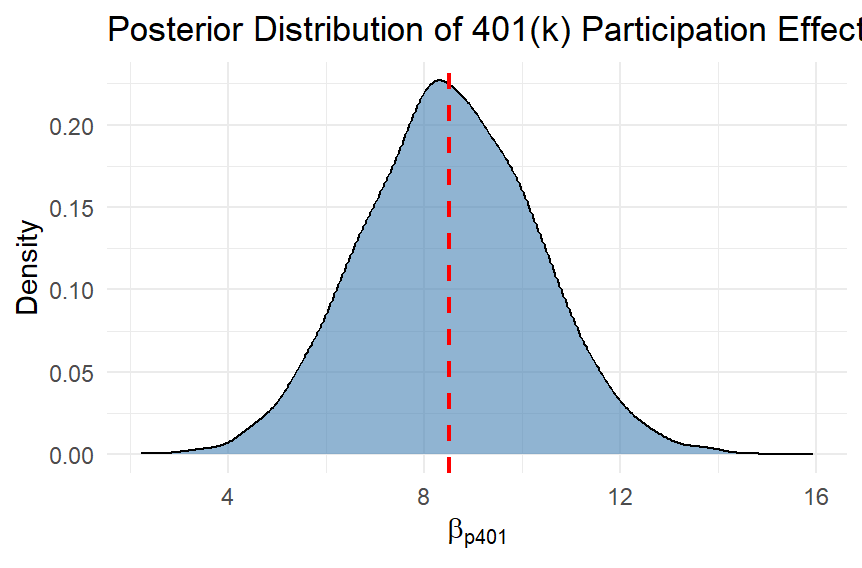
\includegraphics[width=340pt, height=200pt]{Chapters/chapter12/figures/FigP401k.png}
	\caption[List of figure caption goes here]{Posterior distribution: Intention-to-treat effect 401k participation on net financial assets.}\label{fig12_1}
\end{figure}

\item \textbf{401(k) participation on net financial assets continues II} 

Use the function \textit{rivDP} from the \textit{bayesm} package to perform inference on 401(k) participation and its effect on net financial assets using the same specification as in the main text, and plot the LATE.

\textbf{Answer}

The following code implements the exercise, and Figure \ref{fig12_2} display the posterior distribution of the LATE. The results are very similar to the ones in the main text assuming a normal distribution; however, the degree of dispersion of higher using a Dirichlet process for the stochastic errors.  

\begin{tcolorbox}[enhanced,width=4.67in,center upper,
	fontupper=\large\bfseries,drop shadow southwest,sharp corners]
	\textit{R code. Treatment effect: 401(k) participation on net financial assets using Dirichlet process}
	\begin{VF}
		\begin{lstlisting}[language=R]		
rm(list = ls()); set.seed(10101)
library(ggplot2); library(bayesm)
# Load data
mydata <- read.csv("https://raw.githubusercontent.com/BEsmarter-consultancy/BSTApp/refs/heads/master/DataApp/401k.csv",
sep = ",", header = TRUE, quote = "")
# Attach variables
attach(mydata)
y <- net_tfa/1000     # Outcome: net financial assets
x <- as.vector(p401)  # Endogenous regressor: participation
w <- as.matrix(cbind(age, inc, fsize, educ, marr, twoearn, db, pira, hown))  # Exogenous regressors with intercept
z <- as.matrix(e401)  # Instrument: eligibility (NO intercept here)

# specify data input and mcmc parameters
Data = list(); 
Data$z <- z
Data$x <- x
Data$y <- y
Data$w <- w

Mcmc = list()
Mcmc$maxuniq <- 100
Mcmc$R <- 5000
keep <- seq((1000+1), Mcmc$R)

out <- rivDP(Data=Data, Mcmc=Mcmc)

# Plot posterior distribution of treatment effect
df_ITT <- data.frame(ITT = out[["betadraw"]][kepp])
ggplot(df_ITT, aes(x = ITT)) + geom_density(fill = "steelblue", alpha = 0.6) + geom_vline(xintercept = mean(ITT), color = "red", linetype = "dashed", linewidth = 1) + labs(title = "Posterior Distribution of 401(k) ITT: Dirichlet process", x = expression(beta["ITT"]), y = "Density") + theme_minimal(base_size = 14)
\end{lstlisting}
	\end{VF}
\end{tcolorbox} 

\begin{figure}[h!]
	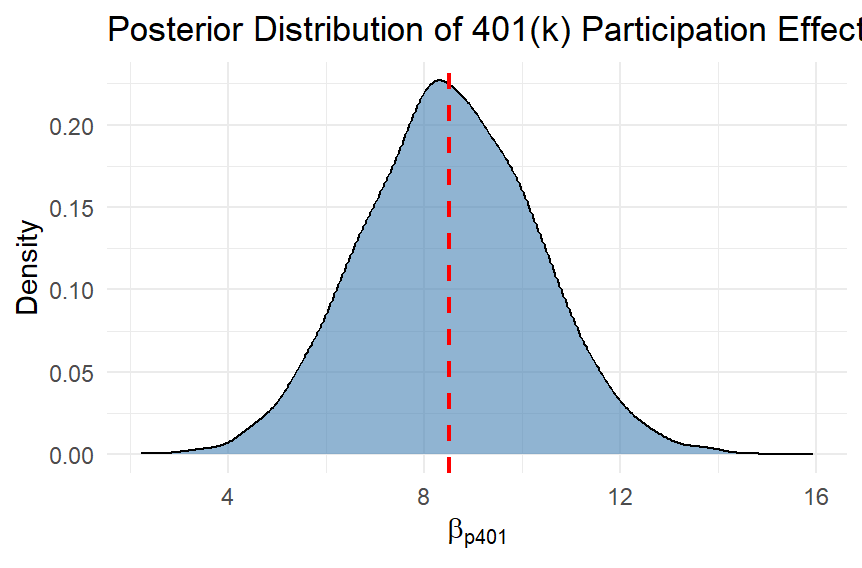
\includegraphics[width=340pt, height=200pt]{Chapters/chapter12/figures/FigP401k.png}
	\caption[List of figure caption goes here]{Posterior distribution: Local average treatment effect 401k participation on net financial assets using a Dirichlet process.}\label{fig12_2}
\end{figure}


\end{enumerate}